\section{The result as a three-layer concept graph}
\label{sec:graph}

\begin{figure*}[t]
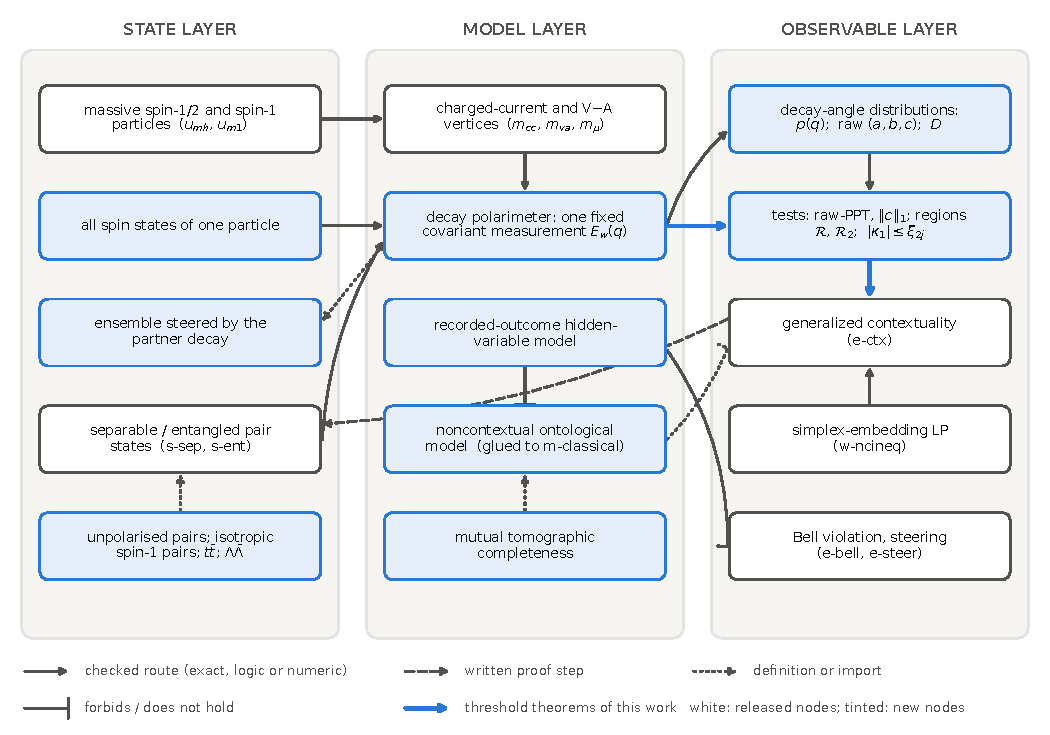
\includegraphics[width=0.86\textwidth]{fig_network}
\caption{The routes of this paper in the three-layer concept graph (condensed: several nodes and routes are merged in each box and arrow; the full list is in Appendix~\ref{app:catalogue}). State layer: what is prepared. Model layer: what assigns probabilities. Observable layer: what is recorded or decided. White boxes are nodes of the released graphs \cite{genhep,gengpt}, tinted boxes are new. The thick arrows are the threshold theorems; the bar-ended line records that the recorded-outcome model forbids Bell violation and steering while it is not a noncontextual model.}
\label{fig:network}
\end{figure*}

The statements of Secs.~\ref{sec:setting}--\ref{sec:apps} are encoded as a graph with three layers. \emph{State} nodes are things that are prepared: particles as representations, sets of spin states, steered ensembles, separable and entangled pair states. \emph{Model} nodes assign probabilities: interaction terms, the Born rule, the decay polarimeter, hidden-variable and ontological models, and assumptions such as tomographic completeness. \emph{Observable} nodes are what is recorded or decided: angular distributions and their coefficients, tests, and effects such as generalized contextuality or Bell violation. There are \nNodes\ nodes (\nS\ state, \nM\ model, \nO\ observable); \nReleased\ keep the identifiers of the released graph of particle physics \cite{genhep} and of the Nonclassicality Network \cite{gengpt} (with links to the resource-theory graph \cite{genqrt}), and \nNew\ are new (Appendix~\ref{app:catalogue}).

A \emph{route} is a statement with input nodes, a target node, a relation (derives, implies, equivalent, forbids, witness, defines) and a grade:
\emph{exact}, an identity or equivalence checked in exact arithmetic by computer algebra \cite{sympy2017};
\emph{logic}, a statement whose negation is shown unsatisfiable by an SMT solver \cite{z3};
\emph{numeric}, a floating-point computation with a stated tolerance \cite{scipy,highs,cvxpy,clarabel}, or the reading of a recorded long run;
\emph{import}, a statement cited from the literature;
\emph{definition}; and
\emph{written}, a proof given in this paper that no program has checked.
Of the \nRoutes\ routes, \nChecked\ carry certificates that are executed (\nExact\ exact, \nLogic\ logic, \nNumeric\ numeric, and \nImportChecked\ import with a consistency check), \nImported\ are imports, \nDefinitions\ are definitions and \nWritten\ are written proofs. No certificate fails.

Each headline claim lists the routes it rests on, and its verdict is the weakest status among them (Table~\ref{tab:claims}). Two claims are verified by executed certificates alone; the theorems are verified modulo the written proofs and the imported simplex-embedding lemma.

\begin{table}[t]
\caption{Headline claims, the routes they rest on, and the verdict of the closure. C1: the decay as a fixed covariant measurement and the $V\!-\!A$ kernels. C2: single-setting data admit a recorded-outcome model that is not noncontextual. C3--C4: Theorems~\ref{thm:half}, \ref{thm:pair}. C5--C6: Theorems~\ref{thm:one}, \ref{thm:onepair}. C7: Theorem~\ref{thm:spinj}. C8--C11: applications to top-quark pairs, hyperon pairs, top-quark polarimeters and vector mesons.}
\label{tab:claims}
\begin{ruledtabular}
\begin{tabular}{lp{0.50\columnwidth}p{0.30\columnwidth}}
Claim & Routes & Verdict \\
\hline
C1 & DV1, DV2, DV3, DV6 & verified modulo written proofs \\
C2 & FW2, FW3, FW4, FW5 & verified \\
C3 & FW1, H1, H2 & verified modulo imports \\
C4 & FW1, DV9, H3, H4, H12, H5, H6, H7, H10 & verified modulo imports and written proofs \\
C5 & FW1, FW6, DV7, V1, V2, V3, V4, V5, V6, P5 & verified modulo imports and written proofs \\
C6 & FW1, FW6, DV7, V1, V2, P1, P2, P3, P6, P4, P5 & verified modulo imports and written proofs \\
C7 & FW1, FW6, G1, G2, G3, G4, G5, G6, G7 & verified modulo imports and written proofs \\
C8 & H6, A1, A2 & verified modulo imports \\
C9 & H3, H4, DV9, A3, A4 & verified modulo imports and written proofs \\
C10 & H1, H2, DV4, DV5 & verified \\
C11 & V3, V5, A7, A8 & verified modulo imports and written proofs \\
\end{tabular}
\end{ruledtabular}

\end{table}

Three further checks are part of the encoding. (i) \emph{Negative controls}: \nControls\ errors are planted in accepted statements (a threshold $1/2$ instead of $1/3$; the opposite sign of the spin vector in Eq.~\eqref{eq:trace}; the Frobenius norm instead of the trace norm in Corollary~\ref{cor:tstate}; a shifted ellipse; a different apex; a wrong coefficient in Eq.~\eqref{eq:m12}; a Euclidean projector in Lemma~\ref{lem:range}; and others), and the corresponding check must reject each; \nControlsRejected\ are rejected. (ii) \emph{Lint}: every observable node is reached by a route from the model layer, every effect node has a witness, and no node is unused. (iii) \emph{Scope separation}: the route ``the recorded-outcome model forbids Bell violation'' and the route ``the recorded-outcome model is not a noncontextual model'' must both be present and certified, so that the conclusion ``no Bell test, yet contextuality is testable'' cannot arise from mixing the two notions.

What the graph contributed is the following. The question was read off as a missing connection between two released graphs. Every theorem is a path across the layers: for Theorem~\ref{thm:pair}, from the entangled-state node through the polarimeter node to the joint distribution, the raw test and the contextuality node, with one back-edge from the model layer to the state layer, since the decay of the partner defines the steered ensemble. Two released edges of the Nonclassicality Network reappear with the measurement fixed: simplex embedding as the definition of classicality, and contextuality as a precondition of entanglement \cite{plavala2024}, which becomes a strict implication (Corollary~\ref{cor:ent}). Finally, the grades separate what was computed from what was proved by hand and from what was cited; this separation is the content of the verdicts and it is not a substitute for a formal proof of the written steps.
